\documentclass[a4paper]{article}
\usepackage[left=2.1cm, right=2.1cm, top=2.1cm]{geometry}
\usepackage{lipsum}
\usepackage{tikzpagenodes}
\usepackage{pgfplots}
\usepackage{tikz}
\usepackage{tikz-3dplot}
\usetikzlibrary{arrows,decorations.pathmorphing,backgrounds,positioning,fit,matrix}
\pgfplotsset{compat=1.8}
\usepackage{graphics} % for pdf, bitmapped graphics files
\usepackage{epsfig} % for postscript graphics files
\usepackage[colorlinks=true,citecolor=green]{hyperref}
\usepackage{cite}
\usepackage{amsmath,amssymb,amsfonts}
\usepackage{algorithmic}
\usepackage{graphicx}
\usepackage{url}
\usepackage{cite}
\usepackage{bm}
\usepackage{pbox}
\usepackage{siunitx,booktabs,etoolbox}
\usepackage{ulem}
\usepackage[framed,numbered,autolinebreaks,useliterate]{mcode}
\usepackage{filecontents}
%\usepackage{bigfoot} % to allow verbatim in footnote


\def\BibTeX{{\rm B\kern-.05em{\sc i\kern-.025em b}\kern-.08em
    T\kern-.1667em\lower.7ex\hbox{E}\kern-.125emX}}


\begin{document}

\title{Exercise on Multiple Images Stiching}
\author{xiahaa@space.dtu.dk}
\maketitle%%

In this exercise, you will work on using all algorithms you have developed yet to do the stiching for more than two images.

\section{Key Steps}
In order to stich more images, you will have several options:
\subsection{Option $1$}
\begin{enumerate}
\item Choose two images and stich them.
\item Use the stiched image and a third image, stich again.
\item Iterate the previous two steps until all images have been added.
\end{enumerate}
The advantage of this option is easy to implement. However, the disadvantage is the complexity will grow significantly when more images have been stiched because you will have one image quite large.

\subsection{Option $2$}
The second option is similar to this tutorial\footnote{\url{https://www.mathworks.com/help/vision/examples/feature-based-panoramic-image-stitching.html}}. 
\begin{enumerate}
	\item load images.
	\item denote previous image as $i-1$ and current image as $i$, detect feature points and descrptors for $i-1$ and $i$, match them, and compute the homography (although in the tutorial, the geometric transformation is used, we can still use homography).
	\item compute the size for the final stiched image (You can use \textbf{maketform, imtransform} and the homography $\mathbf{H}$ to compute the output limits for each image). Then find the bounding box that enclose all stiched images.
	\item find the center of the bounding box and then find the image which will be the nearest one to the center after transformation. Make this image as the base.
	\item When you have the base image, you need recompute the homography relative to this base image. For example, after step $2$, you will have $\mathbf{H}_2^1,\mathbf{H}_3^2, \cdots$. Here the superscript means to which image, subscript means from which image, so $\mathbf{H}_2^1, \cdots$ means the homography from image $2$ to image $1$. Now you set image $3$ as the base, then the homography from image $1$ to image $3$ can be computed as $\mathbf{H}_1^3=(\mathbf{H}_3^2)^{-1}(\mathbf{H}_2^1)^{-1}$ since $\mathbf{H}_1^3=\mathbf{H}_2^3\mathbf{H}_1^2$ and $\mathbf{H}_1^2=(\mathbf{H}_2^1)^{-1}$, $\mathbf{H}_2^3=(\mathbf{H}_3^2)^{-1}$\footnote{If $\mathbf{H}$ is from $i$ to $j$, the $\mathbf{H}^{-1}$ is from $j$ to $i$.}. 
	\item The final step is to warp each image to the stiched image and blend.
\end{enumerate}

\subsection{Option $3$}
In my code \textbf{main\_stich\_mutiple.m}, I am using a different strategy as follows
\begin{enumerate}
	\item load every image, do feature detection and description;
	\item do matching for each pair, there will be $C_n^2$ pairs. You will get a matrix of $n \times n$ with each element denotes how many matches obtained. For example, the $(2,3)$ element contains the number of features matched for image $2$ and image $3$. Note this matrix is symmetric which means $(i,j)==(j,i)$. 
	\item Next, I will treat the  $n \times n$ matrix as a graph and find the minimum spanning tree which will connect all nodes with the minimum cost. 
	\item From that tree, a node will be selected as the root. For others, the shortest path from root node to current node will be found. This gives us the relationship from base to current image.
	\item Compute homography using the corresponding shortest path.
	\item Stich and blend.
\end{enumerate}
The strategy will try to stich images with the order that the feature macthes can reach the maximum. For example, image $1$ and image $2$ have $50$ matches,  image $1$ and image $3$ have $100$ matches,  image $2$ and image $3$ have $300$ matches. Then this method will pick image $2$ as the base and use $3 \to 2$, $1\to3\to2$ as the order to compute new homographies.

\begin{figure*}[!b]
	\centering
	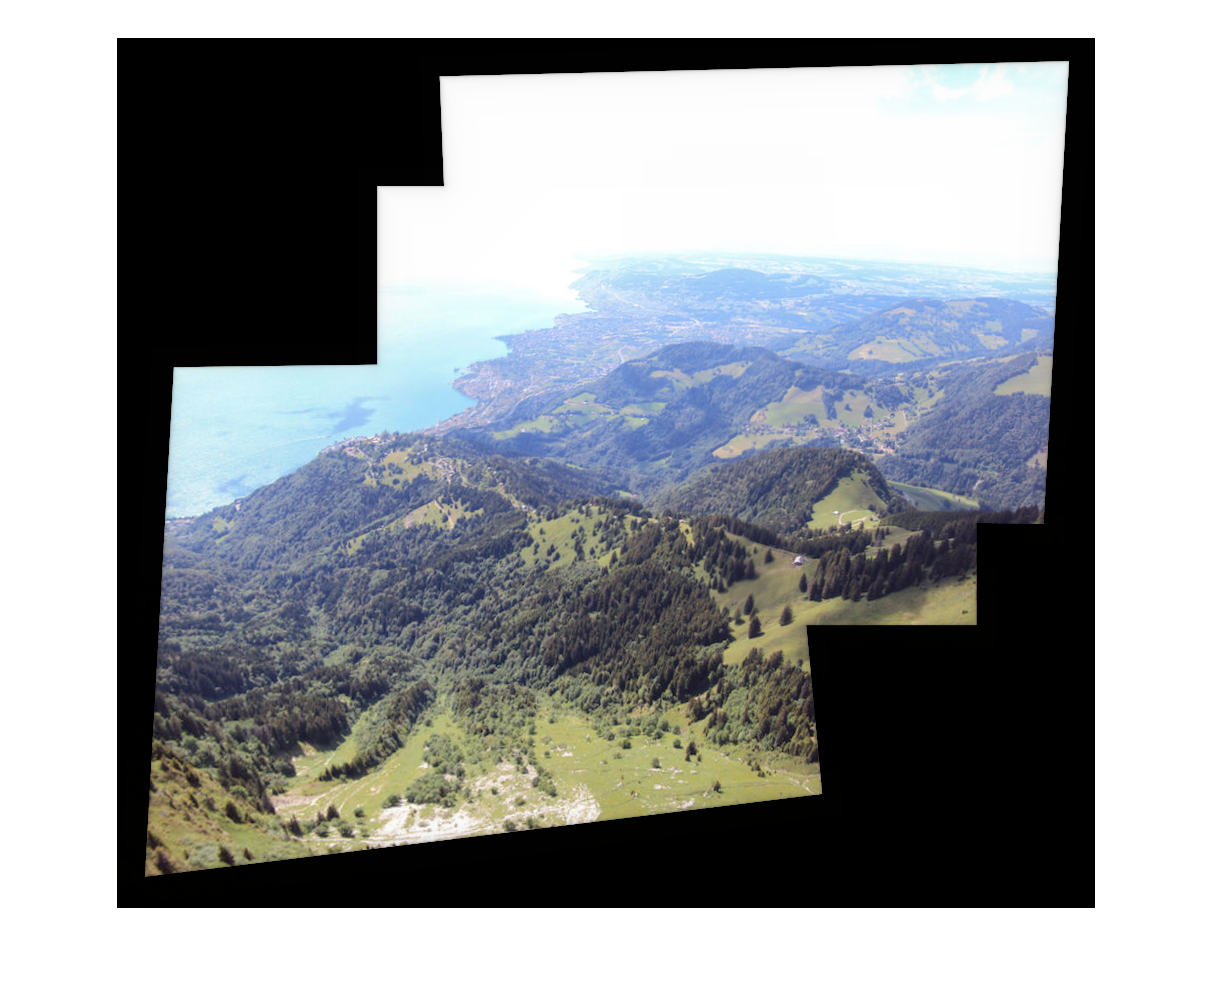
\includegraphics[scale=0.3]{figures/stich_multiple.png}
	\caption{Example of image stich result.}
\end{figure*}

\end{document}